\begin{frame}
  \frametitle{Command memento sheet}
  \begin{columns}
    \column{0.6\textwidth}
    \begin{itemize}
       \item This memento sheet gives command examples for the most
       typical needs (looking for files, extracting a tar archive...)
       \item It saves us 1 day of UNIX / Linux command line training.
       \item Our best tip: in the command line shell, always hit the
       \code{Tab} key to complete command names and file paths.
       This avoids 95\% of typing mistakes.
       \item Get an electronic copy on
       \url{https://bootlin.com/doc/legacy/command-line/command_memento.pdf}
    \end{itemize}
    \column{0.4\textwidth}
    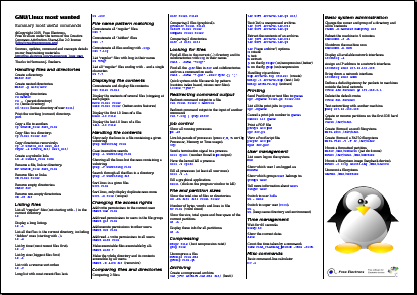
\includegraphics[width=\textwidth]{slides/course-information/command_memento.png}
  \end{columns}
\end{frame}
